\section{Results}

\subsection{FOC Controller Validation}
	
	\subsubsection{Current Status Summary}
	
	Table~\ref{tab:foc_status} summarizes the current status of the FOC 
	controller development.
	
	\begin{table}[htbp]
	\caption{FOC controller development status}
	\label{tab:foc_status}
	\centering
	\begin{tabular}{l c}
	\toprule
	\textbf{Task} & \textbf{Status} \\
	\midrule
	VESC firmware compilation & Completed \\
	Pin compatibility (F405 / L476) & Completed \\
	Schematic design (KiCad) & Completed \\
	ERC validation & Completed \\
	PCB routing & In progress \\
	Tile footprint correction & In progress \\
	Board manufacturing & Planned \\
	Hardware testing & Planned \\
	\bottomrule
	\end{tabular}
	\end{table}

\subsection{Bicycle-Cargo System Control Results}

\subsubsection{Simulation Results}
The closed-loop Simulink model presented in the subsection~\ref{subsec:Simulink_model} was used to evaluate the performance of the proposed PI-based (Proportional-Integral) control strategy.

Figure~\ref{fig:tracking-error} shows the evolution of the tracking error between the bicycle and the cargo cart during simulation. The response exhibits an initial transient phase followed by a progressive convergence toward the desired equilibrium position, demonstrating stable closed-loop behaviour and satisfactory tracking performance.
\begin{figure}[!h]
    \centering 
    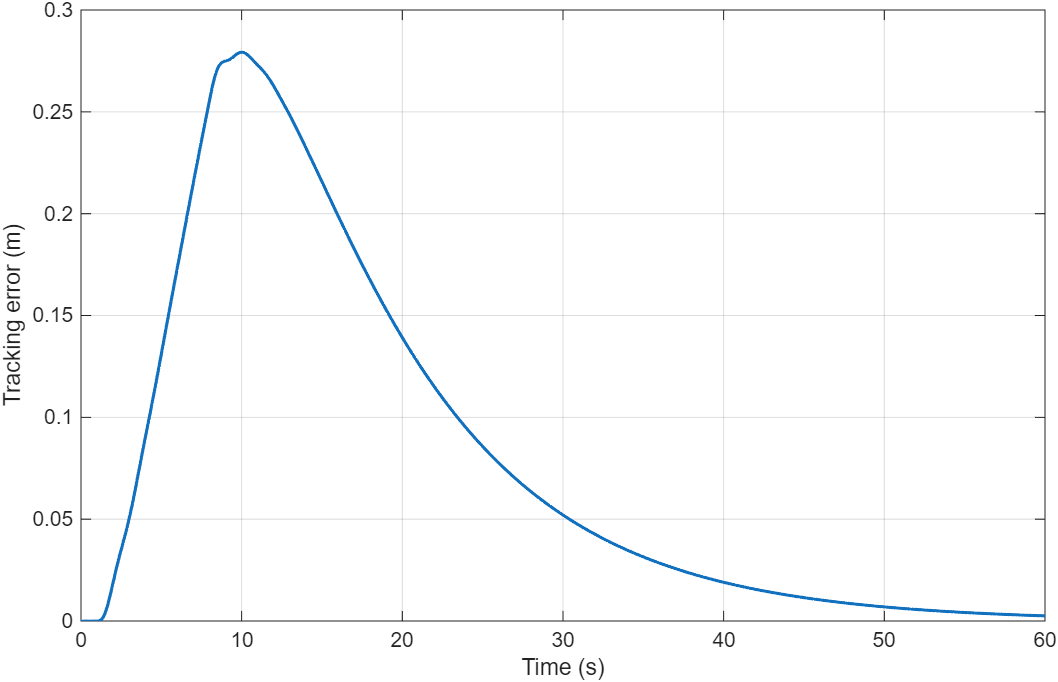
\includegraphics[width=\linewidth]{./Figures/error_fig.png} 
    \caption{Position tracking error between bicycle and cargo cart.} 
    \label{fig:tracking-error} 
\end{figure} 

\subsubsection{Experimental Load Characterization}
Experimental tests were conducted on flat terrain in order to evaluate the influence of mechanical load on the motor current consumption of the cargo cart system. The system was powered using a \SI{48}{\volt} battery pack.

Current measurements were acquired using an Analog Discovery 2 connected to a computer running the WaveForms software environment. A current clamp probe was used to measure the motor current, and the signals were sampled at \SI{1}{\kilo\hertz}.

During each test, the throttle command was set to its maximum value in order to produce the highest possible acceleration. Once the maximum speed was reached, the motor current naturally decreased and stabilised as the motor only compensated for rolling resistance and friction effects.

Three loading conditions were investigated corresponding approximately to one, two, and three passengers inside the cargo cart. The motor current measured during these experiments is shown in Fig.~\ref{fig:motor-currents}.

\begin{figure}[!h]
    \centering 
    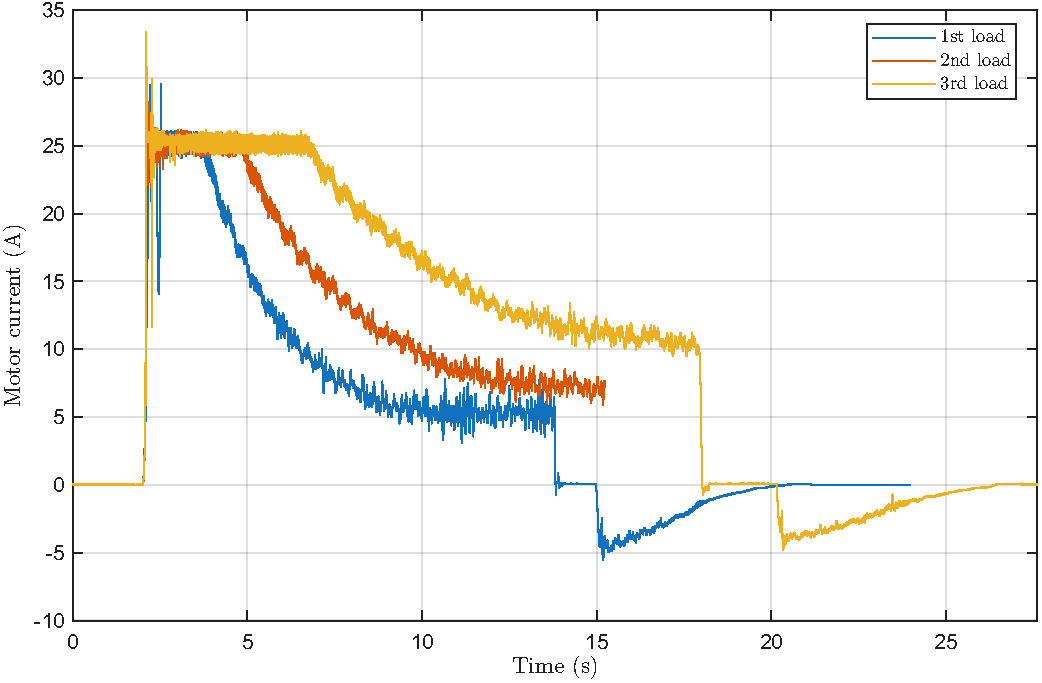
\includegraphics[width=\linewidth]{./Figures/Motor_currents.pdf} 
    \caption{Measured motor current under three loading conditions.} 
    \label{fig:motor-currents} 
\end{figure} 

The results show a significant current peak during the acceleration phase, reaching the controller limit of approximately \SI{25}{\ampere}. After this transient phase, the current decreases and converges toward a lower steady-state value corresponding mainly to friction and resistive force compensation.

As expected, higher loading conditions resulted in higher steady-state current consumption, indicating an increase in the required motor torque. In addition, the duration during which the current remained close to the maximum controller limit also increased with heavier loads, reflecting the longer acceleration time required to reach steady-state operation.
These variations are mainly attributed to terrain irregularities, throttle response fluctuations, and limitations associated with the measurement setup and current probe acquisition chain.

However, due to the absence of direct velocity measurements during the experiments, only qualitative observations could be extracted from these tests. Consequently, a precise estimation of dynamic friction parameters and energy efficiency could not be achieved.

\subsection{FOC Controller Validation}

\subsubsection{Current Status Summary}

Table~\ref{tab:foc_status} summarizes the current status of the FOC controller development.

\begin{table}[htbp]
\caption{FOC controller development status}
\label{tab:foc_status}
\centering
\begin{tabular}{l c}
\toprule
\textbf{Task} & \textbf{Status} \\
\midrule
VESC firmware compilation & Completed \\
Pin compatibility (F405 / L476) & Completed \\
Schematic design (KiCad) & Completed \\
ERC validation & Completed \\
PCB routing & In progress \\
Tile footprint correction & In progress \\
Board manufacturing & Planned \\
Hardware testing & Planned \\
\bottomrule
\end{tabular}
\end{table}


